\documentclass[conference]{IEEEtran}
\IEEEoverridecommandlockouts
% The preceding line is only needed to identify funding in the first footnote. If that is unneeded, please comment it out.
%Template version as of 6/27/2024

\usepackage{cite}
\usepackage{amsmath,amssymb,amsfonts}
\usepackage{algorithmic}
\usepackage{graphicx}
\usepackage{textcomp}
\usepackage{xcolor}
\def\BibTeX{{\rm B\kern-.05em{\sc i\kern-.025em b}\kern-.08em
    T\kern-.1667em\lower.7ex\hbox{E}\kern-.125emX}}



\begin{document}

\title{Conference Paper Title*\\
{\footnotesize \textsuperscript{*}Note: Sub-titles are not captured for https://ieeexplore.ieee.org  and
should not be used}
\thanks{Identify applicable funding agency here. If none, delete this.}
}

\author{\IEEEauthorblockN{1\textsuperscript{st} Daniel Schafhäutle}
\IEEEauthorblockA{\textit{Computational and Data Science} \\
\textit{FHGR}\\
Chur, Switzerland \\
daniel.schafhautle@stud.fhgr.ch}
\and
\IEEEauthorblockN{2\textsuperscript{nd} Joshua Kohler}
\IEEEauthorblockA{\textit{Computational and Data Science} \\
\textit{FHGR}\\
Chur, Switzerland \\
joshua.kohler@stud.fhgr.ch}
\and
\IEEEauthorblockN{3\textsuperscript{rd} Gian-Luca Lanfranchi}
\IEEEauthorblockA{\textit{Computational and Data Science} \\
\textit{FHGR}\\
Chur, Switzerland \\
gianluca.lanfranchi@stud.fhgr.ch}
}

\maketitle

\begin{abstract}
The traveling salesman problem (TSP) is an NP hard combinatorial optimiza-
tion problem, that asks for the shortest possible route that visits a set of cities
and returns to the starting city. Solving TSPs exactly using brute-force meth-
ods quickly becomes computationally infeasible as the number of cities increases.
However, there exists a number of heuristic and metaheuristic algorithms, that
can find reasonably good solutions in a much shorter time. This paper presents
a comparison of five such methods, namely: Simulated Annealing, Tabu Search,
2-Opt, Iterative Local Search and a Genetic Algorithm. Algorithms are evaluated
using benchmark TSP instances of sizes n = [10, 25, 50, 100, 200, 500] with k = 30
instances each. We preform this experiment with two types of instances: one with
uniformly sampled cities and one with clustered cities. They are then compared
based on the solution quality measured as the gap to the optimal solution obtained
by the Concorde TSP solver, and the time required to find the solution. The goal
of this paper is to compare the strengths and weaknesses of these algorithms, that
are the basis of many state of the art methods for solving TSPs and provide a
starting point for further research into this area.
\end{abstract}
\section{Introduction}

The traveling salesman problem (TSP) is a classic combinatorial optimization problem that asks for the shortest possible route that visits a set of cities and returns to the origin city.
More formally, given a complete Graph \( G=(V,E) \), where \( V = \{v_{1},v_{2},\ldots ,v_n\} \) is the set of nodes representing the cities,
and \( d(v_i,v_j) \) is the distance associated with the edge between each pair of nodes \( v_i,v_j \in V \).
A solution to the TSP is an ordering of cities \( (v_{\pi(1)}, v_{\pi(2)}, \ldots  , v_{\pi(n)})\) that minimizes the total tour length:

\begin{equation}
	\left( \sum_{i=1}^{n-1} d(v_{\pi(i)}, v_{\pi(i+1)}) \right) + d(v_{\pi(n)}, v_{\pi(1)})
	\label{eq:tsp-def}
\end{equation}




Complexity: Explain why it matters (NP-hard, combinatorial explosion where brute force requires $O(n!)$ operations).


The Heuristic Objective: Explain that because exact solutions scale terribly, we trade a guarantee of absolute optimality for speed, aiming for "reasonably good" solutions

\section{Related Work}
\textcolor{red}{ready for proofreading}

The TSP is one of the most intensively studied combinatorial optimization problems. 
Its non-determistic polynomial-time hard nature \cite{garey2002computers} makes exact solution methods infeasible for large instances, 
yet the quest for optimal solutions has driven significant progress in both exact and heuristic algorithms.

\paragraph{Exact Solvers}
The most prominent exact solver for the TSP is \textsc{Concorde}, 
which combines cutting-plane methods, branch-and-bound, and linear programming relaxations to certify optimality. 
Applegate et al. \cite{applegateCertificationOptimalTSP2009} demonstrated the power of this approach by certifying an optimal tour through 85,900 cities, 
the largest problem instance in the Traveling Salesman Problem Library (TSPLIB) collection. 
While exact solvers are the gold standard for verifying solution quality, their exponential worst-case complexity limits their applicability to very large instances.

\paragraph{Metaheuristics for the TSP.}
To overcome the limitations of exact methods, researchers have developed a wide range of heuristic and metaheuristic algorithms that can find near-optimal solutions in reasonable time. 
A comprehensive survey of local search and metaheuristics for the TSP is provided by Rego and Glover \cite{regoLocalSearchMetaheuristics}, 
which covers classical local search (2-Opt, 3-Opt) as well as advanced tabu search and ejection chain methods.

Among the most influential metaheuristics, \textit{Simulated Annealing} (SA) introduced the idea of probabilistic acceptance of worsening moves to escape local optima. 

\textit{Tabu Search} (TS), originally proposed by Glover \cite{regoLocalSearchMetaheuristics} and later refined by Gendreau and Potvin \cite{gendreauTabuSearch2019}, 
uses explicit memory structures (tabu lists) to prevent cycling and guide the search. 

\textit{Iterated Local Search} (ILS) \cite{lourencoIteratedLocalSearch2019} builds chains of local optima by perturbing solutions between applications of a local search, 
achieving state-of-the-art performance on many problems. 

\textit{Genetic Algorithms} (GAs) for the TSP are reviewed by Larra{\~n}aga et al. 
\cite{larranagaGeneticAlgorithmsTravelling1999}, and more recent developments,
including the EAX crossover that can find optimal tours for instances with up to 200,000 cities, are discussed by Whitley \cite{whitleyNextGenerationGenetic2019}.

All of these metaheuristics form the basis of the algorithms implemented and compared in this study.
\section{Materials and Methods}


\subsection{2-Opt}
\subsection{Simulated Annealing}
\subsection{Tabu Search}
\subsection{Iterative Local Search}
\subsection{Genetic Algorithm}



\section{Experiments and Results}


Detail exactly how you conducted the experiment so someone else could replicate it
\subsection{Setup}
\subsubsection{Dataset Generation}

\subsubsection{Benchmark}
Mention greedy baseline

\subsubsection{Hardware / Environment}

\subsection{Results}

\begin{itemize}
	\item Performance Metrics
	\item Plots
\end{itemize}

\begin{figure}[H]
	\begin{center}
		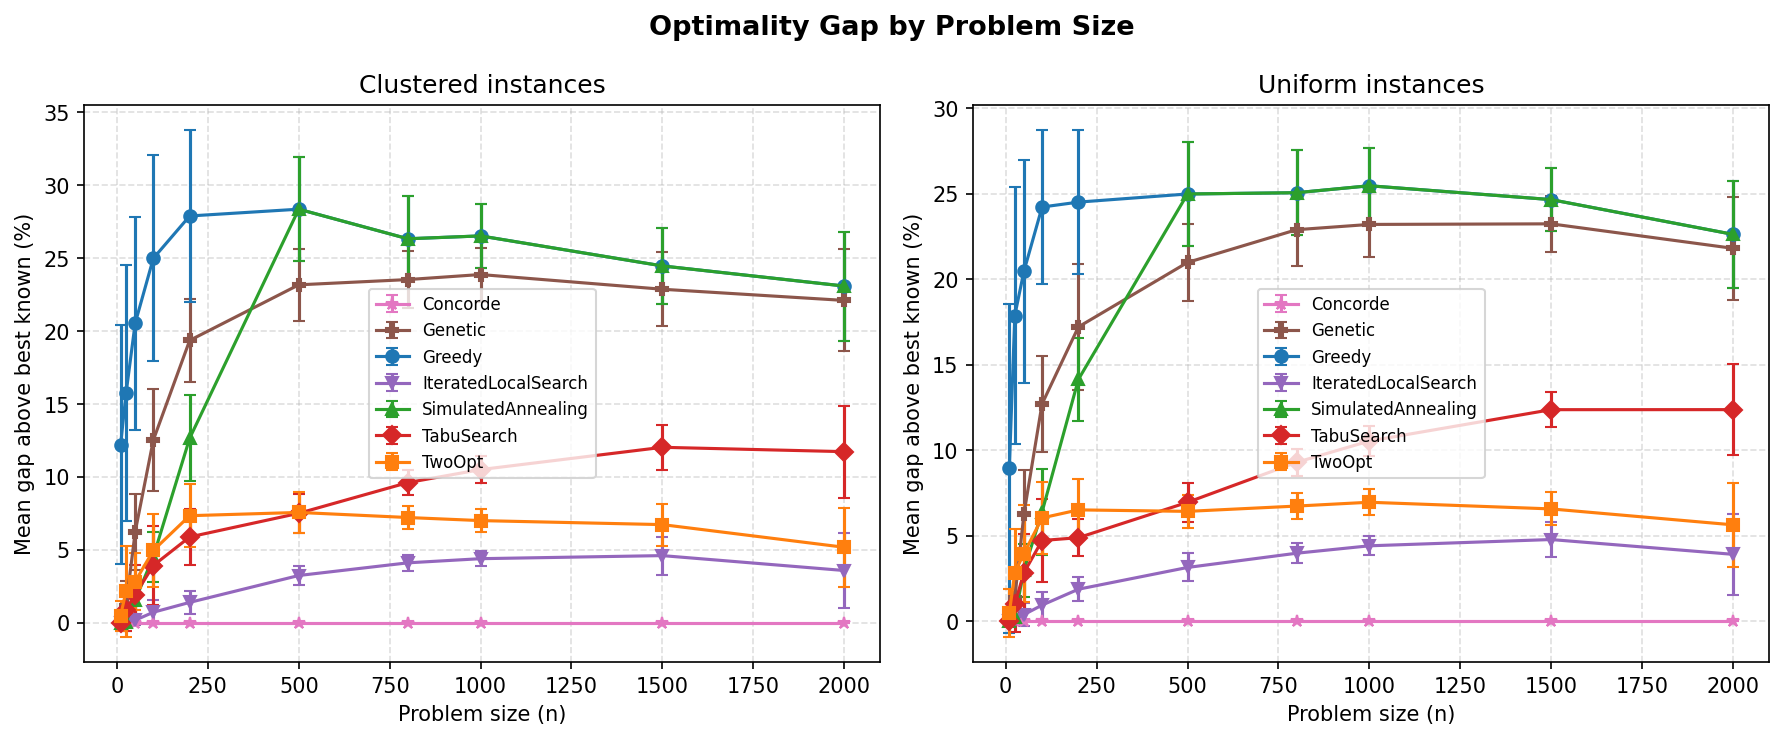
\includegraphics[width=0.95\linewidth]{figures/optimality_gap_lines.png}
	\end{center}
	\caption{Optimality gap of algorithms for different sizes and distributions}\label{fig:optimality_gap_lines}
\end{figure}

\textcolor{red}{Probably split Figure~\ref{fig:optimality_gap_lines} in half, so that it is nicely visible in single column layout.}

\begin{figure}[H]
	\begin{center}
		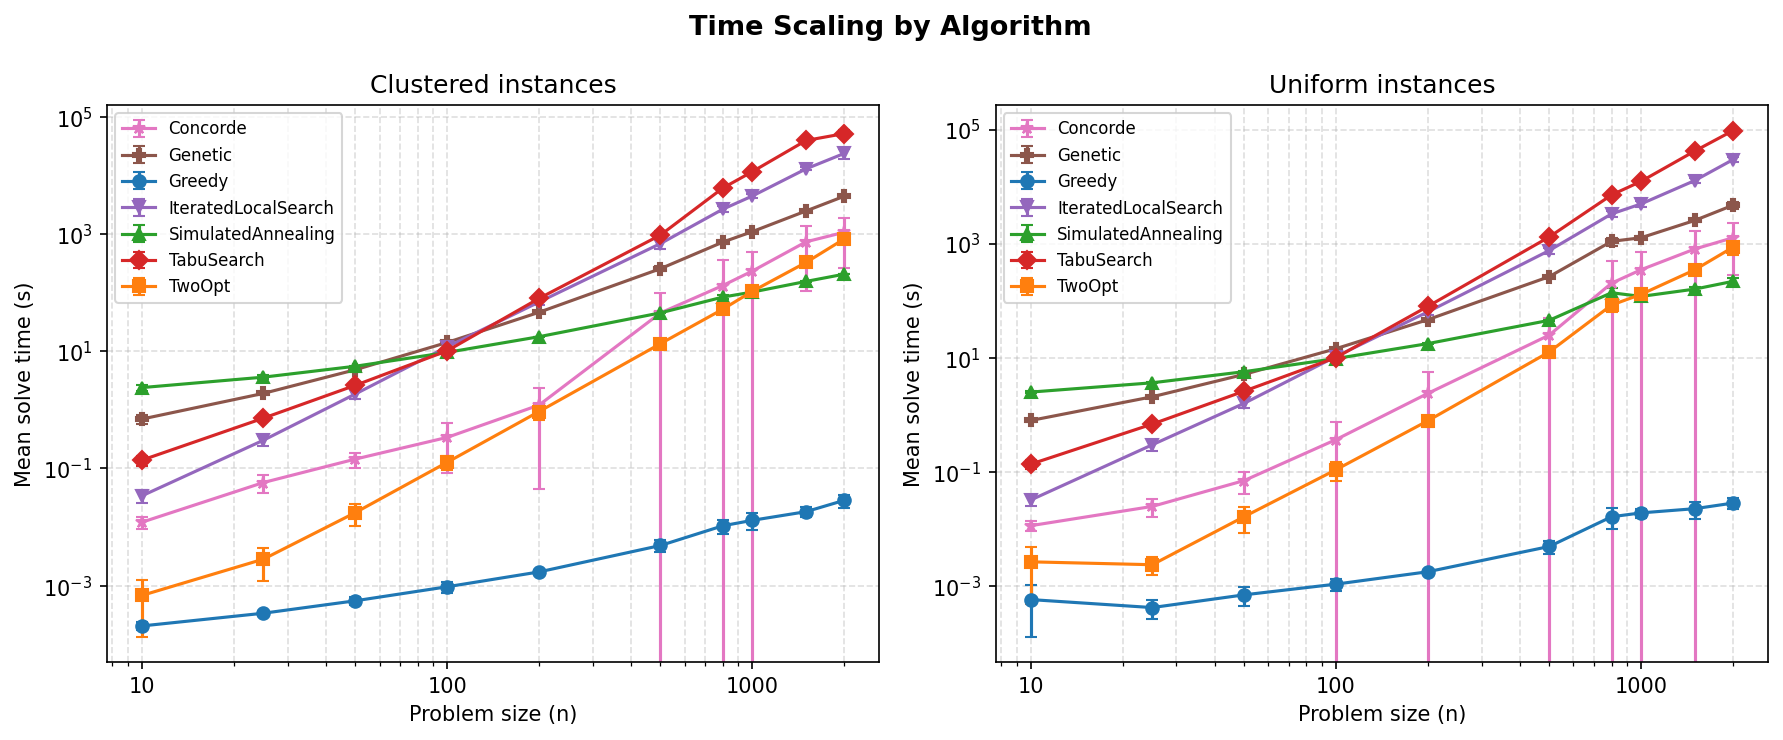
\includegraphics[width=0.95\linewidth]{figures/time_scaling.png}
	\end{center}
	\caption{Time scaling of algorithms for different sizes and distributions.}\label{fig:time_scaling}
\end{figure}


\section{Discussion}

Trade off analysis. Speed vs Quality.

Best all rounder, fast but sloppy, accurate but expensive...

Explain why the results look like that.
Why is one algorithm better able to handle clusters than another. etc.

\section{Conclusion}

We have presented a brief introduction to some of the most important methods to solve the Traveling Salesman Problem using heuristics and metaheuristics.
After explaining the core concepts of these algorithms, we compared them using synthetic TSP instances, ranging in size from 10 to 2000 cities, and examined their scaling behaviour and their differences.
This directly showcases them in a comparable way, providing new researchers in the TSP space with a good sense of how they perform.
After reading this paper, it is our hope that the reader feels empowered to start their own research into TSP algorithms.



\section{Acknowledgement}
The draft of Sections \ref{subsec:tabu-search} and \ref{subsec:genetic} was prepared
with the assistance of DeepSeek \cite{DeepSeekShenDuQiuSuo}, which also helped improve the
English language. The content was reviewed and adjusted to ensure correctness and accuracy.


\textcolor{red}{Wollt ihr die Referenzen manuell oder mit z.B. Zotero machen?}
\begin{thebibliography}{00}
    \bibitem{b1} G. Eason, B. Noble, and I. N. Sneddon, ``On certain integrals of Lipschitz-Hankel type involving products of Bessel functions,'' Phil. Trans. Roy. Soc. London, vol. A247, pp. 529--551, April 1955.
\end{thebibliography}


\input{content/9_appendix.tex}

\end{document}
